\documentclass{resume}
\begin{document}
\fontfamily{ppl}\selectfont
\noindent
% TITLE
\begin{tabularx}{\linewidth}{@{}m{0.75\textwidth} m{0.2\textwidth}@{}} { \Large{\textbf{Alberto
Rota}} \newline
    \small{ \clink{ \href{mailto:alberto_rota@outlook.com}{alberto\_rota@outlook.com} \textbf{|}
        {\fontdimen2\font=0.75ex +39 346 2142 633} } \newline
        Born: $1^{st}$ July 1998 in Bergamo, Italy } } & {
    \hfill
    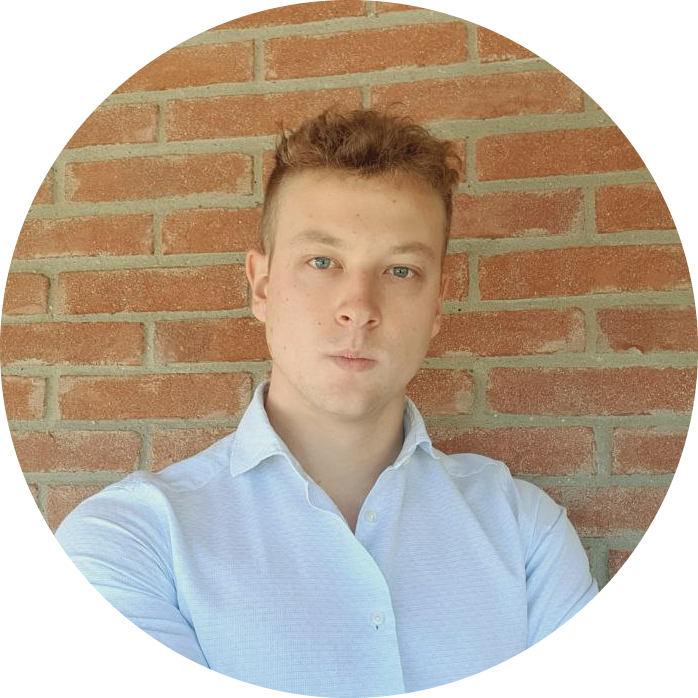
\includegraphics[width=2.5cm]{pic.png}
}
\end{tabularx}
\begin{center}
\begin{tabularx}{\linewidth}{@{}*{2}{X}@{}}
%% LEFT SIDE %%
    % EDUCATION %%
    \csection{EDUCATION \vspace{2.5pt}}{\small
        \begin{itemize}
            \item \frcontent{MSc in Biomedical Engineering - \textit{Ongoing}}{Politecnico di
            Milano, IT}{Thesis:
            \href{https://github.com/alberto-rota/MSc-Thesis-Active-Constraints-in-RAMIS}
            {\textit{Active Constraints in Robot-Assisted Minimally Invasive
            Surgery}} at \href{https://nearlab.polimi.it/}{\textit{NEARLab}}. Supervisor: Prof. Elena de Momi, \textit{PhD}}{\textit{September 2020 -
            expected December 2022}}
            \item \frcontent{Erasmus Exchange Program}{University of Liège, BE}{Joint thesis with
            Politecnico di Milano, visiting fellow at \textit{Multibody  and mechatronics systems
            LAB}}{February 2022 - June 2022}
            \item \frcontent{BSc in Biomedical Engineering, 104/110}{Politecnico di Milano,
            IT}{Thesis:
            \href{https://github.com/alberto-rota/Analisi-delle-Variabilit-di-Reti-Microvascolari-3D-muVES}{\textit{Analysis
            on the 3D variability of in-vitro microvascular networks}}. Supervisors: Prof. Maria
            Laura Costantino, \textit{PhD}; Prof. Luca Possenti, \textit{PhD}}{2017-2020}
            
            \item \frcontent{High School Scientific Diploma}{Lorenzo Mascheroni High School, Bergamo
            IT}{}{2012-2017}
        \end{itemize}
    }

    %% SKILLS %% 
   \csection{SKILLS}{\small
       \begin{itemize}
           \item \textbf{Language} \newline
           {\footnotesize \setlength\itemsep{0.05em} Italian: \textit{Native speaker} \newline
               English: Fluent - \textit{TOEIC Level C1}, 2020 \newline
               French: Elementary - \textit{Level A2+} }
           \item \textbf{Technical}
           \newline
           {\footnotesize Programming: \textit{Python, C++, C, MATLAB, C\#, Git} \newline
               AI: \textit{Tensorflow+Keras framework}\newline
               CAD: \textit{AutoDesk Inventor, Blender}\newline
               Engineering: \textit{ROS, OpenFOAM, ImageJ, Unity}\newline
               Hardware: \textit{Microcontollers, 3Dprinting, KiCAD} }
           \item \textbf{Soft Skills} \newline
           {\footnotesize Problem-solving skills -- Organizational and leadership skills -- Ability
           and propensity to work in a team -- Time-management skills}
       \end{itemize}
   }
%% RIGHT SIDE %%
    & {
    %% MAJOR PROJECTS %%
    \csection{MAJOR PROJECTS}{\small
        \begin{itemize}
            \item  {\href{https://github.com/alberto-rota/muVES}{\textbf{$\mu$VES}} \newline
            A fully automated algorithm for the topo-morphological analysis of 3D microvascular
            networks images from confocal microscopy. \newline \textit{(Research paper pending for
            review)}}

            \item {\href{https://github.com/alberto-rota/ECC-Centifugal-Pump-Tester}{\textbf{ECC
            Pump conformity test}}\newline
            An IR-based embedded device for testing the industrial/commercial conformity of
            centrifugal pumps for extra-corporeal circulation. \newline \textit{Best Development}
            awardee at the 2022 Capstone Project event - In collaboration with \textit{Qura s.r.l.} }

            \item {References for Minor projects are available at
            \href{https://github.com/alberto-rota}{\textit{my GitHub page}}}
            
        \end{itemize} 
        }
    %% PUBLICATIONS %% 
    % \href{https://orcid.org/0000-0001-9609-6294}   
    \csection{RESEARCH}{\footnotesize
        \begin{itemize}
            \item {\textit{A Unity-based Da Vinci Robot Simulator for Surgical Training}: Fan K.,
            Marzullo A., Pasini N., \textbf{Rota A.}, Pecorella M., Ferrigno G., de Momi E. - IEEE
            BioRob2022 [\textit{Review Pending}]}
            \item{\textit{A three-dimensional method for morphological analysis
            and flow velocity estimation in microvasculature on-a-chip}:
            \newline
            \textbf{Rota A.}, Possenti L., Offeddu G.S. ,Senesi M., Stucchi A.,
            Venturelli I.,  Rancati T., Zunino P., Costantino M.L., Kamm R.D. -
            Microvascular Research 
            [\textit{Review Pending}]}
         \end{itemize}
    }
    %% CERTIFICATIONS %%
    \csection{\href{https://github.com/alberto-rota/Certifications}{CERTIFICATIONS}}{\small
        \begin{itemize}
            \item {\footnotesize TOEIC certification for the english language, level C1}
            \item {\footnotesize MATLAB Fundamentals, MATLAB Programming Techniques, MATLAB for Data
            Processing and Visualization from \textit{MathWorks Training}}
            \item {\footnotesize AutoCAD Essential Training, AutoCAD Surface Model Design from
            \textit{LinkedIn Learning}}
        \end{itemize}
    }
    %% PERSONAL INTERESTS %%
    \csection{PERSONAL INTERESTS}{\small
        \vspace{0.32cm}
        \begin{tabularx}{\linewidth}{@{}*{4}{>{\centering\arraybackslash}X}@{}} {\centering
            
\includegraphics[width=0.8cm]{images/bake.png}
            } & {\centering
            
\includegraphics[width=0.8cm]{images/guitar.png}
            } & {\centering
            
\includegraphics[width=0.8cm]{images/plant.png}
            } & {\centering
            
\includegraphics[width=0.8cm]{images/cloud-computing.png}
            } \\
            {\footnotesize Cooking} & {\footnotesize Music} & {\footnotesize Gardening} &
            {\footnotesize IoT} \\
            \vspace{0.20cm}
        \end{tabularx}
    }
    }
\end{tabularx}
\end{center}
\end{document}